% -*- TeX-master: "../fat_manual.tex" -*-

\section{EBL RHUL File Preparation (Beamer)
  \label{makeFile}}
For making the pattern we can either:
\begin{itemize}
\item Crete a full wafer design  in autocad/beamer \ira supply the P,
  Q coordinates \ira perform a full exposure;
\item Design individual  pattern in autocad/beamer \ira  supply P, Q,
  chip  marks, arrays  at JEOL  (see \autoref{subsec:jobMaker})  \ira
  perform exposure.
\end{itemize}

When creating  a full wafer  pattern, we will use  1/4 of a  3" wafer
\red{which we load into a 2" window.}

 \subsection{Autocad}
 To make  patterns for the  lithographer (optical and  electron beam)
 the designs need to be made  in Autocad. Draw whatever you want, but
 follow these rules:

 \begin{itemize}
 \item There must be an object in the zero layer;
 \item All shapes \textbf{must} be  polylines. They must be joined up
   in a single line, or they wont work;
 \item Units are in microns;
 \item \red{Place small markers in the corners of the pattern so that
     centering is correct};
 \item Once  design is finished,  \texttt{select all \ira  Purge \ira
     All \ira type "none*" \ira Yes to all};
 \item Save as \texttt{Autocad DXF} to use it in beamer.
 \end{itemize}

 \begin{framed}\noindent
   Important  is  the  \cmd{extent}  of the  pattern.   This  is  the
   dimensions   that  the   pattern   will  be   overlayed  on   e.g.
   $ 100 \times 100\,\mu$m which we can enlarge, scale etc.

 \begin{center}
   \red{The base dose, relative to which all the dosing is done, will
     need to be experimentally found  by doing test patterns on JEOL.
     Only then do the relative doses that the program makes will mean
     something.}
 \end{center}
\end{framed}

\subsection{General information}
\begin{itemize}
\item Sending is done via \verb|FTP| with \texttt{FileZilla};
\item  Internally,  beamer  uses  its  own  file  format  during  its
  processing;
\item  Double  click   in  bottom  right  symbol   to  view  pattern.
  \cmd{Right  mouse  click}  to   do  measurements.   \cmd{Tick}  and
  \cmd{clear} to retain commands during movement and zooming in;
\item \cmd{Shot settings} button to see dots that JEOL will fire;
\item \cmd{Layout B(oundary)box} button to show extent of pattern;
\item \cmd{Colour by cell} to highlight colours in design;
\item \quote{Doses \ira  Get Limits from Layout}  to recalibrate the
  dose scale;
\end{itemize}

\subsection{How exposure is being done}
\begin{itemize}
\item \verb|JEOL| switches between different fields, `stitching' them
  together;
\item JEOL starts in  the upper left.  Then it fills either  $ X $ or
  $ Y $ direction trapezoids;
\item \textbf{Shot size} = size of  the ciruclar shots that are going
  to be taken  by the Gaussian beam.  Typical is  2-3\,nm, defined by
  the regime of JEOL;
\item \textbf{Shot pitch} = beam step  size as it moves from position
  to position;

\begin{figure}[h]
  \centering 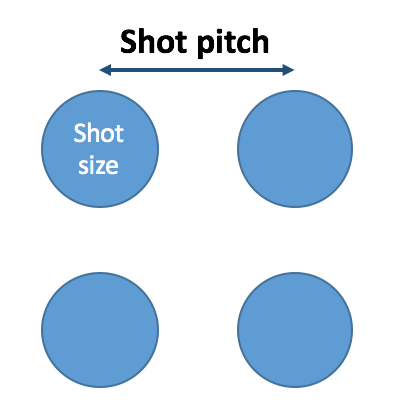
\includegraphics[height=5cm]{jeol_shot}
\end{figure}

\noindent
\item Designs snap onto JEOL grid, which could distort shapes.
  % \item Field changes from 1\,mm to 100\,$ \mu $m,
  %   depending on how little stage movement you
  %   want, and how accurate you want the exposure;
\item Backscattering 35\,$ \mu $m for 100\,keV and silicon;
\end{itemize}
\newpage
\begin{center}
  {\Huge \textbf{BEAMER TIME}!}
\end{center}
\begin{framed}\noindent
  Beamer works in relative doses:
  \begin{itemize}
  \item 1 = no dose modulation;
  \item 0.8 = -20\% of the dose;
  \item 1.2 = + 20\% of the dose;
  \end{itemize}

  \red{\textbf{The final dose depends on your shape, voltage, and the
      shot pitch}}

  To  use variables  in a  for loop,  declare them  in the  transform
  function (for example) instead of a number

  \begin{equation}
    \label{eq:variable}
    Rotate:    \%VARIABLE-NAME\%
  \end{equation}

  \noindent and then increment them in the \textbf{loop} function.
\end{framed}

\subsection{Import}
\begin{itemize}
\item Eats \cmd{dwg} \ira converted to internal file format;
\item \cmd{Convert  colour to  datatype} to  import layers  by colour
  \hfill \red{I do not use};
\item The pattern is centered relative to the most extereme elements;
\end{itemize}

\subsection{Actions}
\begin{itemize}
\item \textbf{Edit}  to allow change of  design.  \red{\textbf{Run it
      standalone to create empty design}};
\item \textbf{Mapping} change layer names  to new ones (or into other
  layers);
\item  \textbf{Heal} removes  overlaps -  \red{\textbf{merges into  1
      layer}};
\item \textbf{Merge} collect different layers;
\item \textbf{Transform} to  position about a chosen  origin e.g. set
  \quote{center} to 0,0. The pattern is done in order of appearance;
\item \textbf{Grid} to put the design on a grid with new dimensions;
\item \textbf{P-XOR} Delete odd number of overlays - \red{can be used
    to check difference between original and processed pattern};
\item  \textbf{Loop} to  repeat  the operations.   Merge results  and
  \quote{heal} to remove overlap;
\item \textbf{FDA} modulate DOSE by layer;
  % \item \textbf{Bias} - sizing of elements;
\item \textbf{Bias}  is used to trim  based on edges. Can  be used to
  remove thin structures;
\item \textbf{PEC} is standard proximity correction;
\item \textbf{Ebeam simulation} is to see how the beam will write;
\item  \textbf{Visual  Job}  is  a  standalone  block  which  we  run
  independently.   It creates  a  text file  that  specifies how  the
  generate the arrays, maybe some scaling of the dose;
\item \cmd{Split tool} to branch out lines;

  \begin{framed}\noindent
    \textbf{To draw line }\newline draw it \ira \quote{export\ira advanced}
    and choose \cmd{reserved line class}
  \end{framed}

\item \textbf{Fracture} how the design  is broken up.  This is passed
  onto proximity correction (which subfractures the fractures)
\item   \textbf{Fracture   \iRa  Advanced}   \ira   (\red{\textbf{see
      below}} Combine floating (fields  are freely positioned) and
  fixed (fields are in a grid)  and apply to different layers. Select
  all layers with *);
\end{itemize}
\subsection{Export}
\begin{enumerate}
\item \textbf{Comma seaparated list} to choose layers to extract.
\item \textbf{Machine type} \cmd{JBX-81000FS};
\item \textbf{File type} is  \cmd{.v30} (changes resolution and field
  size automatically)
  \begin{itemize}
  \item  \cmd{3 -  100kV high  Throughput} \hfill  \red{maximum field
      size is 1mm$ \times1$mm};
  \item  \cmd{6 -  100kV high  resolution} \hfill  \red{maximum field
      size is 100$ \mu $m$ \times100\mu $m};
  \end{itemize}
\item \textbf{Shot settings}  \hfill \red{\textbf{finely spaced shots
      $ \equiv $ small doses on each shot}}.
  \begin{itemize}
  \item \cmd{Pattern unit (resolution)} (depends on the mode, 3 or 6,
    \textbf{fixed by JEOL}). \red{Essentially it is the resolution of
      the grid on which the shots are made}
  \item  \cmd{Shot pitch  (step size)}  is how  much to  separate the
    shots on this grid;
  \end{itemize}
  \red{\textbf{Make sure  you keep  the same shot  pitch in  the JEOL
      machine!  JEOL should prevent incorrect pitches.}}
\item \textbf{Field settings (JEOL moves stage to expose each field)}
  \begin{itemize}
  \item  \textbf{Size}  of each  field  e.g.   1\,mm  $ \times  $1\,mm  is
    \textbf{fixed  by JEOL}  - below  we change  the data  within the
    1\,mm fields, putting and taking away structures, overlapping and
    other shit;
  \item \quote{Advanced \ira fixed} to position fields like a grid;
  \item  \quote{Advanced  \ira floating  field}  to  look for  large
    blocks of items and center the fields on them;
  \item \quote{Advanced \ira manual \ira  view layout} to define you
    own field.   \textbf{Selecting when floating}  \quote{Shift \ira
      draw box  \ira double  click}.  \red{Make  sure box  is smaller
      than the main field};
  \item \quote{Traversal path} to see how exposure will jump between
    the fields;
  \item \quote{Center to field} to make sure that important elements
    are in the field center.
  \end{itemize}
\item \cmd{Shot  pitch factoring} is where  you tell the shots  to be
  perfect on  the edges, and overlap  in the middle of  the structure
  where it is not important;

  \begin{figure}[h]
    \centering 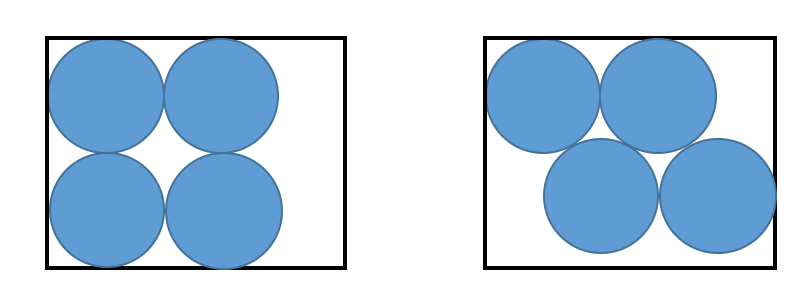
\includegraphics[height=5cm]{jeol_pack}
  \end{figure}

  \noindent
\item  \cmd{Feature  sorting in  field}  how  to  save the  order  of
  elements inside the fields;

  \begin{framed}\noindent
    \cmd{Feature sorting in field} \ira
    \begin{itemize}
    \item  \textbf{By geometry}  to fill  objects wihtout  jumping or
      another option;
    \item \textbf{Left to right};
    \item \textbf{By layer};
    \item  \textbf{Writing regions}  fills in  region by  region, who
      size you set.
    \end{itemize}
  \end{framed}
\end{enumerate}

  \subsubsection{Multipass Tab}
  This is  where you say for  the beam to pass  multiple times across
  the same areas to fix stitching problems
  \begin{enumerate}
  \item \cmd{Field overlap},  so that structures on the  edges of two
    fields are  not directly  cut along the  field lines,  but sorted
    into the left and right sectors;

\begin{figure}[h]
  \centering 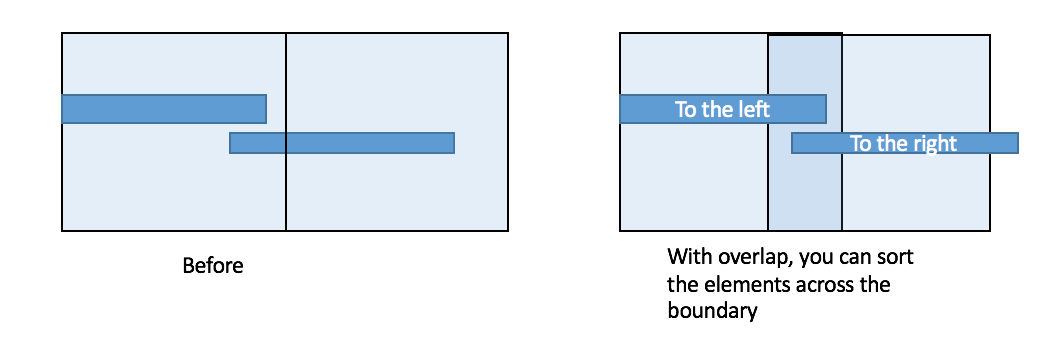
\includegraphics[height=5cm]{jeolOverlap}
\end{figure}

\noindent
% \item  \textbf{For  the  above procedure  use}  \cmd{share  between
%   fields} option;
% \item \cmd{Interleaving fields}  are two combs which  feed into one
%   another, so that you can definitely connect ohmic contacts across
%   two;
\item \cmd{Multipass  shifting and lowering  dose} is when  a pattern
  broken up in  such a way that  the pattern is exposed  4 times, and
  given  1/4 of  the dose  each  time.  Stitches  between fields  are
  smeared out (as they are 1/4 intensity instead of full dose).

\begin{figure}[h]
  \centering 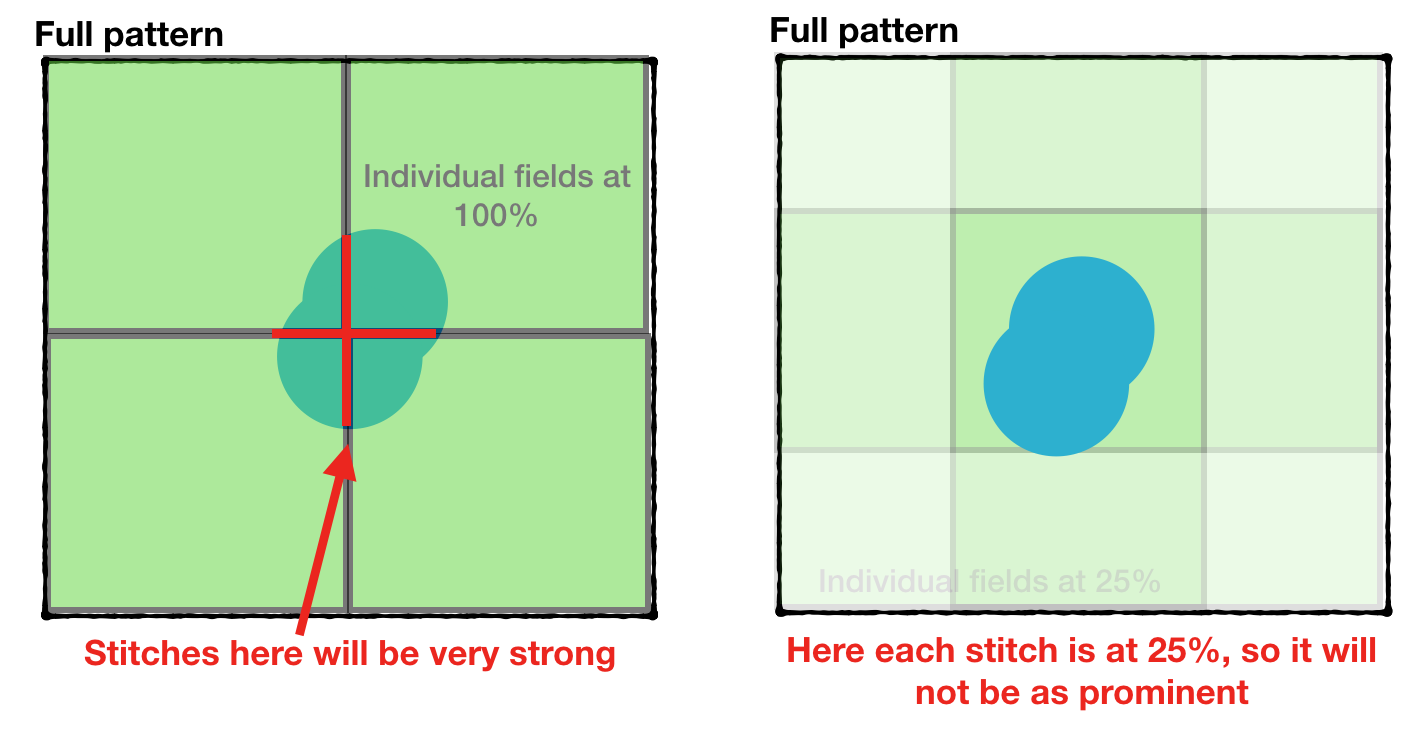
\includegraphics[height=6cm]{stiching_multipass}
\end{figure}

\noindent
\begin{itemize}
\item  Select number  of  passes  and the  overlap  in  terms of  the
  mainfield dimensions. 0.5 is a good value.
\item  \red{Remember  the size  of  the  subfield  (sub part  of  the
    mainfield)  should not  be an  factor of  the mainfield  size, or
    periodicity will appear at integer multiples.}
\end{itemize}
\end{enumerate}

\subsubsection{Improve field movement}
\label{sec:impr-field-movem}
For improved movement of microscope do the following:
\begin{enumerate}
\item Get pattern and \textbf{bias} it to grow a rectangle around it;
\item  \textbf{Merge}  to the  original  pattern  -  now you  have  a
  rectangle layer positioned on top of your pattern.
\item  In export,  select \red{\textbf{region-layer}}  to choose  the
  layers that will specify the centers of the respective fields.  The
  machine  will  move to  those  rectangles,  and look  for  exposure
  patterns there.
\end{enumerate}

 \subsection{Increasing speed}
 To increase  speed, we need to  draw the outline accurately,  and do
 the filling at a larger current. Thus  we need an outline and a fill
 design:

 \begin{itemize}
 \item  \cmd{Bias}   function  will   take  your  pattern   and  trim
   (e.g. 100\,nm) from all edges;
 \item \cmd{MINUS}  this pattern  from the original  \ira you  get an
   outline of the original pattern;
 \item Then  take another  \cmd{bias} and add  (e.g.  50\,nm)  to the
   first  bias to  create overlap  between the  cut out  bias pattern
   (outline)  and the  middle pattern.   \begin{figure}[h] \centering
     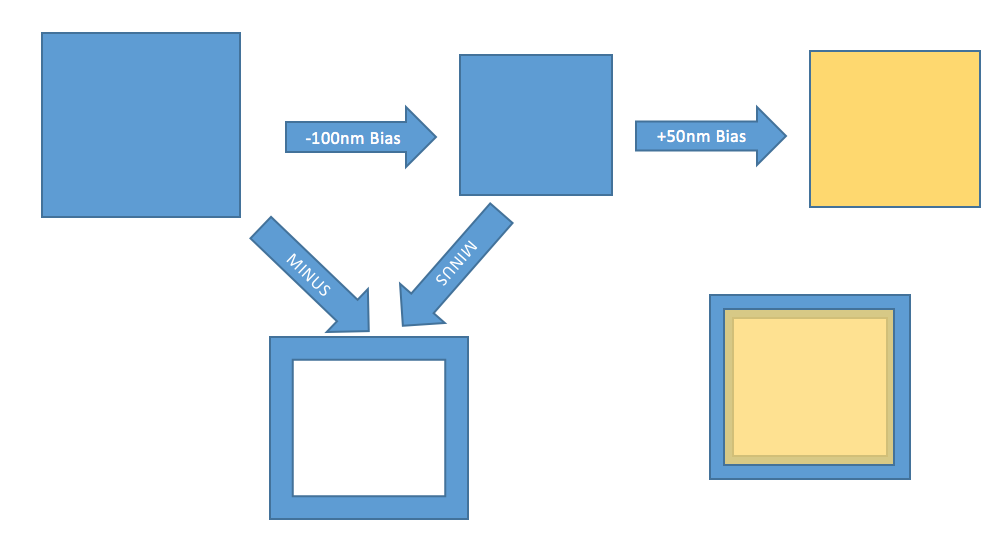
\includegraphics[height=7cm]{jeol_frame}
   \end{figure}

   \noindent
 \end{itemize}

 \subsection{Proximity correction}
 \red{Uses \cmd{Tracer} which we do not have}

 \begin{itemize}
   % \item The proximity correction functions are in
   %   \quote{GenSys \ira Tracer \ira 2DArchive};
 \item \red{Long range correction is always being done!}  Pixel based
   approach. It measure the local density, in  the range of $ \beta $ and
   performs a correction based on this extra exposed dose;
 \item \cmd{Archive} to select
   \begin{enumerate}
   \item Substrate e.g. Silicon+200nm PMMA;
   \item Z-position to  set the position where  the correction should
     be the best (could be  top of bottom of resist).  \red{\textbf{0
         for top of resist}}
   \end{enumerate}
 \item \cmd{``Accuracy''} should be 1\%.
 \item Tick \cmd{Include Short Range Correction} for small structures
   $  \sim  30\,$nm,  where  the  size of  the  onset  beam  can  affect
   neighboring patterns.  Off by default;
 \item \cmd{Effective short-range dose};
 \item  \cmd{Maximum  number  of  dose  classes}  is  the  number  of
   different doses.  \cmd{Accuracy} sets  the accuracy that are given
   to the  dose classes.  Too  much accuracy fractures the  design to
   assign these different doses, \textbf{\red{so do not overdo it}};
 \item \cmd{Minimum dose} exists so that  beam does not jump too fast
   (low dose, means beam can move across this area very fast);

\begin{framed}\noindent
  \cmd{Isodose  grid} defined  the fidelity  of the  grid to  be used
  \red{\ira  \textbf{make sure  that the  \cmd{Shot Pitch}  is larger
      than the  grid so that  you don't have 10\,nm  fractures, which
      you fill with 6\,nm shot steps}}
\end{framed}

\item \cmd{Minimum figure size} sest  the finest fracture that can be
  made.
\item  \quote{Examples}  \ira  \verb|TenDoses_100um_200um.fbd|  that
  allows  to expose  a set  of test  patterns, which  can be  used to
  calibrate  you  own  material   (for  future  proximity  correction
  values).
\end{itemize}

\subsection{Visual-Job - prepare for exposure }
\label{sec:visual-job-add}

To open,  click on the icon  in the toolbar in  BEAMER (multiple dose
tables created)  \red{\textbf{or use the CHIP  PLACE COMMAND} (single
  dose table created)}
\begin{enumerate}
\item Set the marks;
\item Create job name - \red{\textbf{must be capital letters}};
\item \textbf{Shot pitch};
\item \textbf{Array}
  \begin{enumerate}
  \item Set the extent of the pattern slightly larger;
  \item Center the pattern;
  \item \textbf{Array dose} (start + end  e.g.  0.8 to 1.2, linear) -
    separate \cmd{.jdi} files are created;
  \item Open \quote{Place data in the side menu bar};
  \item \textbf{Pattern Data} to set the marker.
  \item \quote{Assign} to put the marker on the pattern.
  \end{enumerate}
\end{enumerate}

\newpage
\subsection{Compiling on RedHat}
\begin{center}
  \begin{itemize}
  \item {\cmd{v30} files are created  in \cmd{beamer} and contain the
      \textbf{geometry} of the pattern;}
  \item {\cmd{jdi} files are created  in \cmd{beamer} and contain the
      \textbf{doses} for the pattern;}
  \item {\cmd{jdf} files  are created in \cmd{Jod  Editor} and create
      \textbf{arrays} of  v30 patterns  and \textbf{assign  doses} to
      them.}
  \end{itemize}
\end{center}
\vspace{1cm}
\begin{enumerate}
\item Create  an jeol  exposure program in  \quote{\cmd{Jod Editor}}
  \ira \cmd{\quote{File \ira  Save As} \ira} save this  project as a
  folder;
\item Copy the \quote{\cmd{.jdi}} files into this folder;
\item Open \quote{\cmd{terminal}} and run the command
  \begin{center}
    \cmd{./jeolrhul}
  \end{center}
\item  Navigate to  the jeol  exposure program  folder created  using
  \cmd{cd} e.g.
  \begin{center}
    \cmd{cd ilya/2018files/transmonnpc}
  \end{center}
\item Run a  script to apply a modulation of  +0\% $ \cdots$+100\% of
  the dose in the \cmd{.jdi file} across:

  \begin{framed}\noindent
    \[
      \begin{aligned}
        \parbox{6cm}{\color{gray} Array number 2 \newline(as it appears in the jdf file)}& \quad  & &\text{\cmd{jeolrhul\_modulate\_array} \quad 2 \quad 100 \quad doseFile.jdi}^{*}\\\\
        \parbox{6cm}{\color{gray} All arrays that use pattern A \newline (as set in \quote{Jod Editor})}& & &\text{\cmd{jeolrhul\_modulate\_pattern} \quad A \quad 100 \quad doseFile.jdi}^{*}\\
      \end{aligned}
    \]
    \hfill  The specifier  $  ^{*}  $ is  only  needed  if there  are
    multiple jdi files files in the folder.
  \end{framed}

\item Compile  the program  in \quote{\cmd{Jod Editor}}  by clicking
  the black arrow $ \blacktriangleright $\newline  \red{\textbf{Do not save} as it will
    overwrite the \cmd{.jdf} file.}
\end{enumerate}

\newpage
